\documentclass[xcolor=pdftex,dvipsnames,table,aspectratio=169]{beamer}
\usetheme{metropolis}
%\usetheme{Darmstadt}
%\usepackage{times}
%\usefonttheme{structurebold}

\usepackage[english]{babel}
%\usepackage[table]{xcolor}
\usepackage{pgf,pgfarrows,pgfnodes,pgfautomata,pgfheaps}
\usepackage{amsmath,amssymb,setspace}
\usepackage[latin1]{inputenc}
\usepackage[T1]{fontenc}


\setbeamercovered{dynamic}

\newcommand{\Lang}[1]{\operatorname{\text{\textsc{#1}}}}

\newcommand{\Class}[1]{\operatorname{\mathchoice
  {\text{\sf \small #1}}
  {\text{\sf \small #1}}
  {\text{\sf #1}}
  {\text{\sf #1}}}}

\newcommand{\NumSAT}      {\text{\small\#SAT}}
\newcommand{\NumA}        {\#_{\!A}}

\newcommand{\barA}        {\,\bar{\!A}}

\newcommand{\Nat}{\mathbb{N}}
\newcommand{\Set}[1]{\{#1\}}

\newcommand{\abs}[1]{\lvert#1\rvert}
\newcommand{\norm}[1]{\lVert#1\rVert}

\pgfdeclaremask{tu}{beamer-tu-logo-mask}
\pgfdeclaremask{computer}{beamer-computer-mask}
\pgfdeclareimage[interpolate=true,mask=computer,height=2cm]{computerimage}{beamer-computer}
\pgfdeclareimage[interpolate=true,mask=computer,height=2cm]{computerworkingimage}{beamer-computerred}
\pgfdeclareimage[mask=tu,height=.5cm]{logo}{beamer-tu-logo}


\begin{document}
\title{MPEC notes}
\author{Chris Conlon\\
 thanks to Che-Lin Su}
\institute{Grad IO}
\date{\today}
\footnotesize
\frame{\titlepage}

\frame{\frametitle{Unconstrained Optimization}
Basic idea in many estimation problems is to use Newton-type methods to solve FOCs of equilibrium or estimating equations
\begin{eqnarray*}
\min f(x) : x \in \mathbb{R}^n
\end{eqnarray*}
\begin{itemize}
\item $f : R^n \rightarrow R, c : R^n \rightarrow R^m$ smooth (typically $\mathcal C^2$)
\item $x \in \mathbb{R}^n$ finite dimensional (may be large)
\end{itemize}
Want to find a local minimizer 
\begin{eqnarray*}
\nabla f(x^{*}) = 0
\end{eqnarray*}
Optimization Algorithms generate a sequence $x^{(k)}$ such that the gradient test
\begin{eqnarray*}
|| \nabla f(x^{(k)}) || \leq  \alert{\tau}
\end{eqnarray*}
is satisfied for some tolerance $\alert{\tau} = 1e-6$ or so.
\alert{Warning!}
}
\frame{\frametitle{General NLP Problem}
A Nonlinear Programming (NLP) problem is defined by:
\begin{eqnarray*}
\begin{cases}
\min_x f(x) \quad \mbox{objective}\\
\mbox{subject to} \quad c(x) = 0 \quad \mbox{constraints}\\
x \geq 0 \quad \mbox{variables}
\end{cases}
\end{eqnarray*}
Typical assumptions
\begin{itemize}
\item $f : R^n \rightarrow R, c : R^n \rightarrow R^m$ smooth (typically $\mathcal{C}^2$)
\item $x \in R^n$ finite dimensional (perhaps large)
\item more general $l \leq c(x) \leq u$ is possible
\end{itemize}
}

\frame{\frametitle{Optimality Conditions for NLP}
\begin{block}{Constraint Qualifications (CQ)}
Linearization of $c(x)= 0$ characterizes all feasible permutations, $x^{*}$ local minimizer \& CQ holds $\exists$ multipliers $\lambda^{*},\gamma^{*}$:
\begin{eqnarray*}
\nabla f(x^*) - \nabla c(x^*) \lambda^* - \gamma^* &=& 0\\
c(x^*) = &=& 0\\
\alert{X^* \lambda^* }&=& 0\\
\alert{x^* \geq 0,\gamma^* }&\geq& 0
\end{eqnarray*}
Where $X^* = diag(x^*)$, thus $X^*\lambda^* = 0 \Leftrightarrow x_i^* \gamma_i^* = 0$
\end{block}
\begin{block}{NLP Solvers}
$F(w) = 0$ where $w = (x,\lambda,\gamma)$ with $x \geq 0, z \geq0$.
Optimization Algorithms generate a sequence $w^{(k)}$ such that the gradient test
\begin{eqnarray*}
|| \nabla f(w^{(k)}) || \leq  \alert{\tau}
\end{eqnarray*}
is satisfied for some tolerance $\alert{\tau} = 1e-6$ or so. (Same \alert{warning}).
\end{block}
}
%\frame{\frametitle{First Steps in Solving an Estimation Model}
%\begin{outline}[enumerate]
%\1 Make sure you have a smooth formulation for the model
%\1 smooth objective function
%\1 smooth constraints
%\2 Use the best available NLP solvers!
%\2 Many free NLP solvers are crappy; they often fail or even worse, can
%give you wrong solutions
%\2 Do not attempt to develop numerical algorithms/solvers by yourself
%\2 You should use solvers developed by professionals", i.e., numerical
%optimization people
%\2 Best NLP solvers: SNOPT (Stanford), KNITRO (Northwestern),
%Filter-SQP (Argonne), IPOPT (IBM), PATH (UW-Madison
%\end{outline}
%}

\frame{\frametitle{Optimization}
\begin{block}{``Folk Theory'' of Optimization in Economics}
\begin{itemize}
\item Unconstrained Optimization is easier than Constrained Optimization 
\item More parameters are harder
\item Quasi-Newton Methods are unreliable
\end{itemize}
\end{block}
\begin{alertblock}{Consequences of Folk Theory}
\begin{itemize}
\item Rewrite all problems as unconstrained optimization
\item Use fixed points and multi-step procedures to reduce parameter space
\item Use Nelder-Mead/Simplex methods for optimization
\end{itemize}
\end{alertblock}
}

\frame{\frametitle{Optimization}
Thanks to recent advances in optimization:
\begin{block}{More Accurate Description of Optimizaiton}
\begin{enumerate}
\item \textit{Shape} of the problem is what matters -- convexity is really important
\item Constrained Problems are not much more difficult
\item More parameters can make the problem \alert{easier} (or harder)
\end{enumerate}
\end{block}
\begin{alertblock}{Consequences of State of the Art Optimization}
\begin{itemize}
\item Tested stable Newton-routines are very reliable.
\item Good Solvers handle 10,000+ parameters
\item Computational burden are Jacobian and Hessian (and storage)
\end{itemize}
\end{alertblock}
}


\frame{\frametitle{Recent Advances in Optimization Literature}
Large Scale Algorithms
\begin{itemize}
\item Much focus has been on very large convex optimization problems -- these have gotten really good.
\item Most of these rely on first and second derivatives and quadratic approximations.
\item Ways to do derivatives: analytic, numeric, symbolic and automatic (new!)
\item Easy to solve 10,000+ parameter constrained problems often in less than 20 major iterations.
\item Lots of industrial strength software packages.
\item When in doubt express your problem as a convex one.
\item Algorithm is polynomial $\approx O(k^3)$
\end{itemize}
}

\section{Convexity}
\frame{\frametitle{Convexity}
\begin{block}{An optimization problem is convex if}
\begin{eqnarray*}
\min_{x} f(\mathbf{x}) &s.t.& h(\mathbf{x}) \leq 0 \quad A \mathbf{x} = 0
\end{eqnarray*}
\vskip -2ex
\begin{itemize}
\item $f(\mathbf{x}),h(\mathbf{x)}$ are convex (PSD second derivative matrix)
\item Equality Constraint is affine
\end{itemize}
\end{block}
\begin{exampleblock}{Some helpful identities about convexity}
\begin{itemize}
\item Compositions  and sums of convex functions are convex.
\item Norms $||$ are convex, $\max$ is convex, $\log$ is convex
\item  $ \log(\sum_{i=1}^n \exp(x_i))$ is convex.
\item Fixed Points can introduce non-convexities.
\item Globally convex problems have a unique optimum
\end{itemize}
\end{exampleblock}
}

\frame{\frametitle{Nested Logit Model}
\begin{exampleblock}{FIML Nested Logit Model is Non-Convex}
\begin{eqnarray*}
\min_{\theta} \sum_j q_j \ln P_j(\theta) \quad \mbox{s.t.} \quad  P_j(\theta) = \frac{e^{x_j \beta/ \lambda}( \sum_{k \in g_l} e^{x_j \beta/ \lambda})^{\lambda-1}}{\sum_{\forall l'} ( \sum_{k \in g_l'} e^{x_j \beta/ \lambda})^{\lambda} }
\end{eqnarray*}
This is a pain to show but the problem is with the cross term $\frac{\partial^2 P_j}{\partial \beta \partial \lambda}$ because $\exp[x_j \beta / \lambda]$ is not convex.
\end{exampleblock}
\begin{exampleblock}{A Simple Substitution Saves the Day:  let $\gamma = \beta / \lambda$}
\begin{eqnarray*}
\min_{\theta} \sum_j q_j \ln P_j(\theta) \quad \mbox{s.t.} \quad  
P_j(\theta) = \frac{e^{x_j \gamma}( \sum_{k \in g_l} e^{x_j \gamma})^{\lambda-1}}{\sum_{\forall l'} ( \sum_{k \in g_l'} e^{x_j \gamma})^{\lambda} }
\end{eqnarray*}
This is much better behaved and easier to optimize.
\end{exampleblock}
}

\frame{\frametitle{Nested Logit Model (Conlon Mortimer AEJ 2013)}
\begin{center}
\rowcolors[]{1}{RoyalBlue!10}{RoyalBlue!20} 
\begin{tabular}{lrrr}
&\bf{Original}\footnote{KNITRO-AMPL} & \bf{Substitution}\footnote{KNITRO-AMPL} & \bf{No Derivatives}\footnote{fminunc-MATLAB} \\
Parameters &49& 49&49\\
Nonlinear $\lambda$ &5 &5 &5\\
Neg LL & 2.279448 &2.279448  & 2.27972\\
Iterations &197 &146 & 352\\
Time & 59.0 s & 10.7 s & 192s  \\
\end{tabular}
\end{center}
Discuss Simplex, Sparsity.
}


\section{MPEC}
\frame{\frametitle{Extremum Estimators}
Often faced with extremum estimator problems in econometrics (ML, GMM, MD, etc.)  that look like:
\begin{eqnarray}
\label{extremum}
\hat{\theta} = \arg \max_{\theta} Q_n(\theta), \quad  \theta \in \Theta
\end{eqnarray}
Many economic problems contain constraints, such as: market clearing (supply equals demand), consumer's consume their entire budget set, or firm's first order conditions are satisfied.  A natural way to represent these problems is as constrained optimization.
}

\frame{\frametitle{Constrained Problems}

\begin{block}{MPEC}
\begin{eqnarray*}
\label{MPEC}
\hat{\theta} = \arg \max_{\theta,P} Q_n(\theta,P), \quad  \mbox{ s .t. } \quad \Psi(P,\theta) =0,  \quad \theta \in \Theta
\end{eqnarray*} 
\end{block}
\pause
\begin{block}{Fixed Point / Implicit Solution}
In much of the literature the tradition has been to express the solutions $\Psi(P,\theta) =0$ implicitly as $P(\theta)$:
\begin{eqnarray*}
\label{NFXP}
\hat{\theta} = \arg \max_{\theta} Q_n(\theta,P(\theta)),  \quad \theta \in \Theta
\end{eqnarray*}
\end{block}
}

\frame{\frametitle{Rust Problem}
\begin{itemize}
\item Bus repairman sees mileage $x_t$ at time $t$ since last overhaul
\item Repairman chooses between overhaul and normal maintenance
\begin{eqnarray*}
u(x_t, d_t, \alert{\theta^c}, \alert{RC}) =
\begin{cases} -c(x_t,\alert{\theta^c}) \quad &\mbox{if} \quad d_t=0\\
-(\alert{RC} + c(0,\alert{\theta^c}) \quad) &\mbox{if} \quad d_t =1\\
\end{cases}
\end{eqnarray*}
\item Repairman solves DP:
\begin{eqnarray*}
V_{\alert{\theta}} (x_t) = \sum_{f_t,f_{t+1},\ldots} E \left\{  \sum_{j=t}^{\infty} \beta^{j-t}   [u(x_j,f_j,\alert{\theta}) + \varepsilon_{j}(f_j)]| x_t \right\}
\end{eqnarray*}
\item Econometrician
\begin{itemize}
\item Observes mileage $x_t$ and decision $d_t$ but not cost.
\item Assumes extreme value distribution for $\varepsilon_t(d_t)$
\end{itemize}
\item Structural parameters to be estimated $\alert{\theta = (\theta^c, RC, \theta^p)}$.
\begin{itemize}
\item Coefficients of cost function $c(x,\alert{\theta^c}) = \theta^c_1 x + \theta^c_2 x^2$
\item Overhaul cost $\alert{RC}$
\item Transition probabilities in mileages $p(x_{t+1} | x_t, d_t, \alert{\theta^p})$
\end{itemize}
\end{itemize}
}


\frame{\frametitle{Rust Problem}
\begin{itemize}
\item Data: time series $(x_t,d_t)_{t=1}^T$
\item Likelihood function
\begin{eqnarray*}
\mathcal{L}(\theta) &=& \prod_{t=2}^T P(d_t | x_t, \alert{\theta^c}, \alert{RC}) p(x_t | x_{t-1}, d_{t-1},\alert{\theta^p})\\
\mbox{ with }  P(d | x, \alert{\theta^c}, \alert{RC}) &=& \frac{\exp[u(x,d,\alert{\theta^c},\alert{RC}) + \beta \textcolor{blue}{EV}_{\alert{\theta}}(x,d)}
{\sum_{d' \in \{0,1\}} \exp[u(x,d',\alert{\theta^c},\alert{RC}) + \beta \textcolor{blue}{EV}_{\alert{\theta}}(x',d)}\\
\textcolor{blue}{EV}_{\alert{\theta}}(x,d) &=& T_{\alert{\theta}}(\textcolor{blue}{EV}_{\alert{\theta}})(x,d)\\
\end{eqnarray*}
\vspace{-1cm}
\begin{eqnarray*}
\equiv \int_{x'=0}^{\infty} &\log& \left[ \sum_{d' \in \{0,1\}} \exp[u(x,d',\alert{\theta^c},\alert{RC}) + \beta \textcolor{blue}{EV}_{\alert{\theta}}(x',d)]  \right] p(dx' | x,d,\alert{\theta^p}) 
\end{eqnarray*}
\end{itemize}
}


\frame{\frametitle{Rust Problem}
\begin{itemize}
\item Outer Loop: Solve Likelihood
\begin{eqnarray*}
\max_{\alert{\theta} \geq 0} \mathcal{L}(\theta) &=& \prod_{t=2}^T P(d_t | x_t, \alert{\theta^c}, \alert{RC}) p(x_t | x_{t-1}, d_{t-1},\alert{\theta^p})\\
\end{eqnarray*}
\item Convergence test: $\norm{\nabla_{\theta} \mathcal{L}(\alert{\theta})} \leq \alert{\epsilon_{out}}$
\item Inner Loop: Compute expected value function $ \textcolor{blue}{EV}_{\alert{\theta}}$ for a given $\alert{\theta}$
\item $ \textcolor{blue}{EV}_{\alert{\theta}}$ is the implicit expected value function defined by the Bellman equation or the fixed point function
\begin{eqnarray*}
 \textcolor{blue}{EV}_{\alert{\theta}} = T_{\alert{\theta}}( \textcolor{blue}{EV}_{\alert{\theta}})
\end{eqnarray*}
\item Convergence test: $\norm{ \textcolor{blue}{EV}^{(k+1)}_{\alert{\theta}} - \textcolor{blue}{EV}^{(k)}_{\alert{\theta}} } \leq \alert{\epsilon_{in}}$
\item Start with contraction iterations and polish with Newton Steps
\end{itemize}
}

\frame{\frametitle{NFXP Concerns}
\begin{itemize}
\item Inner-loop error propagates into outer-loop function and derivatives
\item NFXP needs to solve inner-loop exactly each stage of parameter search
\begin{itemize}
\item to accurately compute the search direction for the outer loop
\item to accurately evaluate derivatives for the outer loop
\item for outer loop to converge!
\end{itemize}
\item Stopping rules: choosing inner-loop and outer-loop tolerance
\begin{itemize}
\item inner loop can be slow: contraction mapping is linearly convergent
\item tempting to loosen inner loop tolerance $\alert{\epsilon_{in}}$ (such as $1e-6$ or larger!).
\item Outer loop may not converge with loose inner loop tolerance.
\begin{itemize}
\item check solver output message
\item tempting to loosen outer loop tolerance $\alert{\epsilon_{out}}$ to promote convergence ($1e-3$ or larger!).
\end{itemize}
\end{itemize}
\end{itemize}
}

\frame{\frametitle{Stopping Rules}
\begin{itemize}
\item $\mathcal{L}(\textcolor{blue}{EV}(\alert{\theta},\alert{\epsilon_{in}} ), \alert{\theta} )$ the programmed outer loop objective function
\item $L$: the Lipschitz constant (like modulus) of inner-loop contraction mapping
\item Analytic derivatives $\nabla_{\theta} \mathcal{L}(\textcolor{blue}{EV}(\alert{\theta},\alert{\epsilon_{in}} ), \alert{\theta} )$ is provided: $\alert{\epsilon_{out}} = O(\frac{L}{1-L} \alert{\epsilon_{in}})$
\item Finite-difference derivatives are used: $\alert{\epsilon_{out}} = O ( \sqrt{\frac{L}{1-L}} \alert{\epsilon_{in}} )$ 
\end{itemize}
}

\frame{\frametitle{Stopping Rules}
\begin{itemize}
\item Form the augmented likelihood function for data $X = (x_t, d_t)_{t=1}^T$
\begin{eqnarray*}
\mathcal{L}(\textcolor{blue}{EV}, \alert{\theta}; X) &=& \prod_{t=2}^T P(d_t | x_t, \alert{\theta^c}, \alert{RC}) p(x_t | x_{t-1}, d_{t-1},\alert{\theta^p})\\
\mbox{ with }  P(d | x, \alert{\theta^c}, \alert{RC}) &=& \frac{\exp[u(x,d,\alert{\theta^c},\alert{RC}) + \beta \textcolor{blue}{EV}(x,d)}
{\sum_{d' \in \{0,1\}} \exp[u(x,d',\alert{\theta^c},\alert{RC}) + \beta \textcolor{blue}{EV}(x',d)}\\
\end{eqnarray*}
\item Rationality and Bellman equation imposes a relationship between $\alert{\theta}$ and $\textcolor{blue}{EV}$
\begin{eqnarray*}
\textcolor{blue}{EV} = T(\textcolor{blue}{EV},\alert{\theta})
\end{eqnarray*}
\item Solve constrained optimization problem
\begin{eqnarray*}
\max_{(\alert{\theta},\textcolor{blue}{EV})} \mathcal{L}(\textcolor{blue}{EV}, \alert{\theta}; X)\\
\mbox{ subject to }  \textcolor{blue}{EV} = T(\textcolor{blue}{EV},\alert{\theta})
\end{eqnarray*}
\end{itemize}
}

\frame{\frametitle{Results}
\begin{figure}[htbp]
\begin{center}
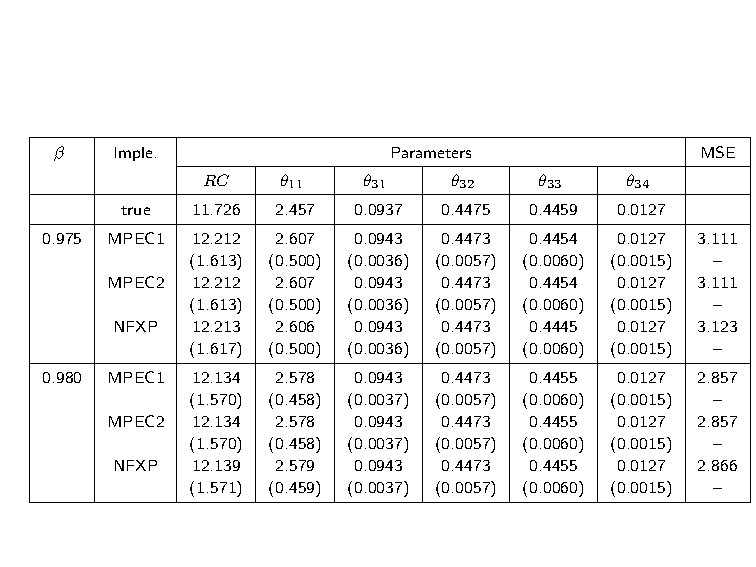
\includegraphics[width=4.5in]{resources/su1.pdf}
\label{default}
\end{center}
\end{figure}
}

\frame{\frametitle{Results}
\begin{figure}[htbp]
\begin{center}
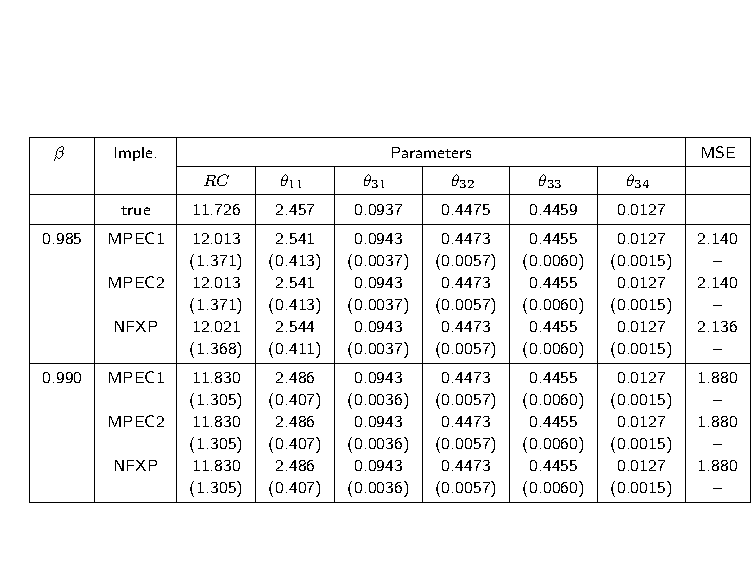
\includegraphics[width=4.5in]{resources/su2.pdf}
\label{default}
\end{center}
\end{figure}
}
\frame{\frametitle{Results}
\begin{figure}[htbp]
\begin{center}
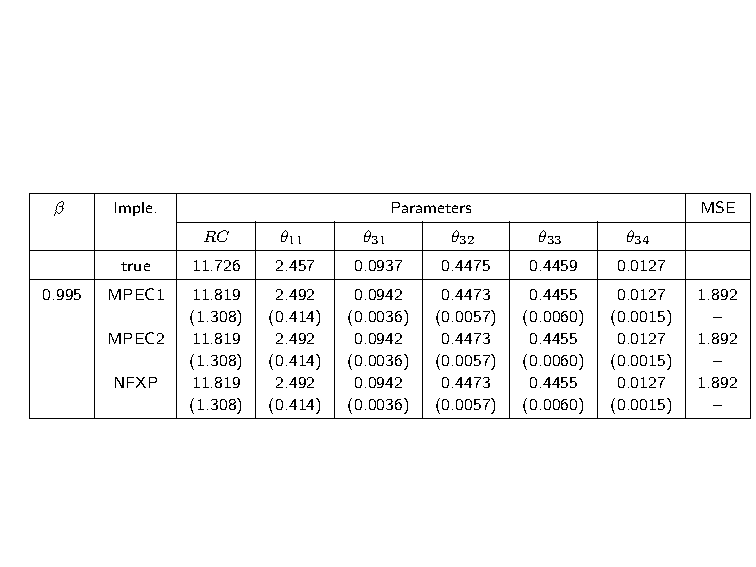
\includegraphics[width=4.5in]{resources/su3.pdf}
\label{default}
\end{center}
\end{figure}
}
\frame{\frametitle{Results}
\begin{figure}[htbp]
\begin{center}
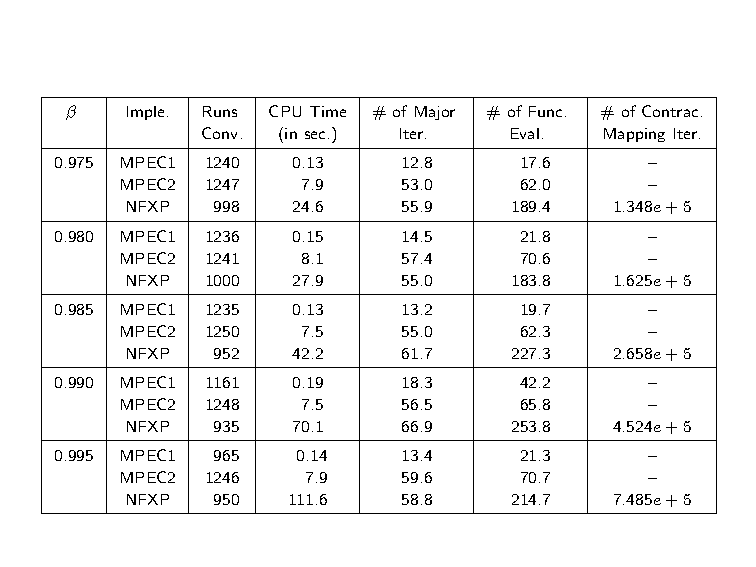
\includegraphics[width=4.5in]{resources/su4.pdf}
\label{default}
\end{center}
\end{figure}
}
\frame{\frametitle{Results}
\begin{figure}[htbp]
\begin{center}
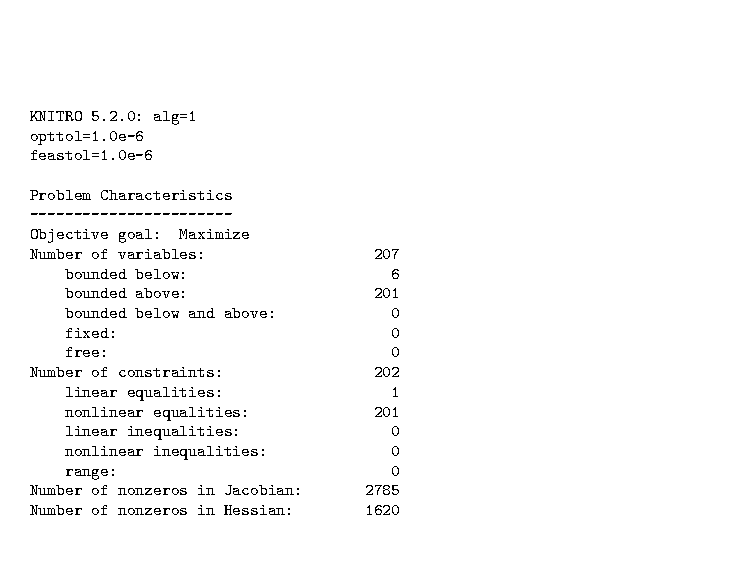
\includegraphics[width=2.5in]{resources/su5.pdf}
\label{default}
\end{center}
\end{figure}
}
\frame{\frametitle{Results}
\begin{figure}[htbp]
\begin{center}
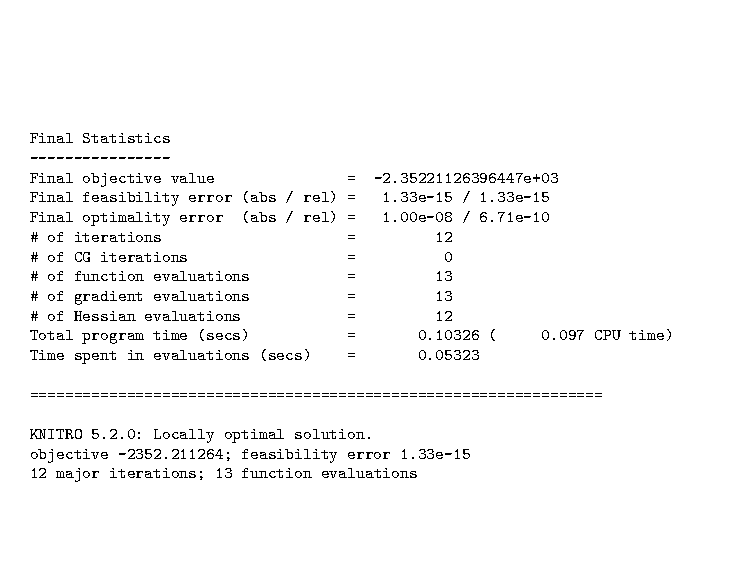
\includegraphics[width=4.5in]{resources/su6.pdf}
\label{default}
\end{center}
\end{figure}
}

\frame{\frametitle{BLP Demand Example}
\begin{exampleblock}{BLP 1995}
The estimator solves the following mathematical program:
\begin{eqnarray*}
\label{blpnfxp}
\min_{\alert{\theta_2}} && g(\xi(\alert{\theta_2}))' W g(\xi(\alert{\theta_2})) \quad \mbox{ s.t. } \\
g(\xi(\alert{\theta_2})) &=& \frac{1}{N} \sum_{\forall j,t} \xi_{jt} (\alert{\theta_2}) ' z_{jt} \\
\xi_{jt}(\alert{\theta_2}) &=& \delta_j(\alert{\theta_2}) - x_{jt} \beta - \alpha p_{jt} \\
s_{jt}(\delta(\alert{\theta_2}),\alert{\theta_2}) &=& \int \frac{\exp[\delta_j(\alert{\theta_2})+ \mu_{ij}]}{1+\sum_k \exp[\delta_j(\alert{\theta_2})+ \mu_{ik}]} f(\mu | \alert{\theta_2})\\
\log(S_{jt})  &=& \log(s_{jt}(\delta(\alert{\theta_2}),\alert{\theta_2})) \quad \forall j,t
\end{eqnarray*}
\end{exampleblock}
}

\frame{\frametitle{BLP Algorithm}
The estimation algorithm is generally as follows:
\begin{enumerate}
\item Guess a value of nonlinear parameters $\alert{\theta_2}$
\item Compute $s_{jt}(\delta,\alert{\theta_2})$ via integration
\item Iterate on $\delta_{jt}^{h+1}  = \delta_{jt}^h +  \log(S_{jt}) - \log(s_{jt}(\delta^{h},\alert{\theta_2}))$ to find the $\delta$ that satisfies the share equation
\item IV Regression $\delta$ on observable $X$ and instruments $Z$ to get residual $\xi$.
\item Use $\xi$ to construct $g(\xi(\alert{\theta_2}))$.
\item Possibly construct other errors/instruments from supply side.
\item Construct GMM Objective
\end{enumerate}
The idea is that $\delta(\alert{\theta_2})$ is an implicit function of the nonlinear parameters $\alert{\theta_2}$. And for each guess we find that implicit solution for reduce the parameter space of the problem.
}

\frame{\frametitle{Dube Fox Su 2009}
\begin{exampleblock}{BLP-MPEC}
The estimator solves the following mathematical program:
\begin{eqnarray*}
\label{blpmpec}
\min_{\alert{\sigma,\alpha,\beta, \xi}}  && g(\alert{\xi})' W g(\alert{\xi}) \quad \mbox{ s.t. } \\
g(\alert{\xi}) &=& \frac{1}{N} \sum_{\forall j,t} \alert{\xi_{jt}'} z_{jt} \\
s_{jt}(\alert{\sigma,\alpha,\beta, \xi}) &=&  \sum_i w_i \frac{\exp[x_{jt} \alert{\beta} + \alert{\xi_{jt}} - \alert{\alpha} p_{jt} + \sum_l \nu_{il} x_{jt}^l \alert{\sigma_l} ] }
{1+ \sum_k \exp[x_{kt} \alert{\beta} + \alert{\xi_{kt}} - \alert{\alpha} p_{kt} + \sum_l \nu_{il} x_{kt}^l \alert{\sigma_l} ]} \\
\log(S_{jt})  &=& \log s_{jt}(\alert{\sigma,\alpha,\beta, \xi}) \quad \forall j,t
\end{eqnarray*}
\end{exampleblock}
\begin{itemize}
\item Expand the parameter space of the nonlinear search to include $\alert{\alpha,\beta,\xi}$
\item Don't have to solve for $\xi$ except at the end.
\item No implicit functions of $\theta_2$
\item Sparsity!
\end{itemize}
}



\section{Empirical Likelihood}
\subsection{Motivation}
\frame{\frametitle{Empirical Likelihood Methods}
\begin{block}{Empirical Likelihood often statistically better than GMM }
\begin{itemize}
\item Higher order efficiency (gets to semi-parametric efficiency bound faster) (Kitamura 2001, 2006)
\item No problems in estimating the weight matrix (Altonji Segal 1995, Newey Smith 2004).
\item Likelihood based units for testing
\item No problems with scaling of parameters / instruments.
\item GMM prone to non-identification in finite-sample (Dominguez Lobato 2004)
\end{itemize}
\end{block}
}

\subsection{Description}
\frame{\frametitle{EL as NPMLE (Owen 1990, Kitamura 2006)}
\begin{block}{Nonparametric MLE}
\begin{equation}
l_{NP} (p_1,\ldots,p_n) = \sum_{i=1}^n \log p_i \quad (p_1,\ldots,p_n) \in \Delta
\end{equation}
\begin{itemize}
\item Observed $z_i$ are IID with measure  $\mu$
\item Simplex defined as $(p_1,p_2,\ldots,p_n) \in \Delta $ such that $\sum_{i=1}^n p_i = 1$ and $p_i \geq 0$
\item Trivial max at $p_i = \frac{1}{n}$ and $\mu_n = \frac{1}{n} \sum_{i=1}^n \delta_{z_i}$ and $l_{NP} = -n \log n$
\end{itemize}
\end{block}
}

\frame{\frametitle{Adding moment conditions}
(Owen 1990) Shows we can extend NPMLE to moment condition models.
\begin{eqnarray*}
E[g(z_i, \theta)] = \int g(z,\theta) d \mu = 0 \in \mathbb{R}^q , \quad \theta \in \Theta \in \mathbb{R}^k
\end{eqnarray*}
This exactly follows our definition of an MPEC problem:
\begin{block}{Empirical Likelihood Estimator}
\begin{eqnarray*}
\arg \max_{\theta, p} l_{NP} &&\\
 l_{NP} = \sum_{i=1}^n \log p_i \quad && \mbox{ s.t. } \quad \sum_{i=1}^n p_i g(z_i,\theta) = 0 \quad \mbox{ and } \sum_{i=1}^n p_i =1
\end{eqnarray*}
\end{block}
}

\begin{frame}
\frametitle{Alternative-Generalized Minimum Contrast}
Idea is to look for a statistical model $\mathcal{P}$ close to the true measure $\mu$
\begin{eqnarray*}
\mathcal{P}(\theta) &=& \{ P \in M : \int g(z,\theta) dP = 0 \}\\
\mathcal{P} &=& \cup_{\theta \in \Theta} \mathcal{P}(\theta) 
\end{eqnarray*}
We do this by minimizing the contrast function $D(P,U) = \int \phi(p) d \mu$ with  $p = \frac{d P}{d \mu}$.
\begin{eqnarray*}
\inf_{\theta \in \Theta} \rho (\theta,\mu) \mbox{  where } \rho(\theta,\mu) = \inf_{P \in \mathcal {P}} D(P,\mu)
\end{eqnarray*}
Produces (infinite dimensional) constrained problem:
\begin{eqnarray*}
v(\theta) = \inf_p \int \phi(p) d \mu \quad  \int g(z,\theta) p d \mu = 0 \quad \int p d \mu = 1
\end{eqnarray*} 
Choose a contrast function $\phi(x) = \log(x)$ (EL) or $\phi(x) = \frac{1}{2}(x^2-1)$ (CUE)
\end{frame}


\frame{\frametitle{Interpreting EL}
Simple Alternate Explanation
\begin{itemize}
\item GMM asks what are the parameters $\theta$ that minimize the quadratic distance under some metric $A$ between my model applied to the observed data, and my model in the ``ideal'' case. (Model generally doesn't hold exactly -- overidentified).
\item EL asks how different a distribution of data would I need to observe in order to meet the implications of my model.
\item EL as solutions to systems of equations (which one do we pick?)
\item Now I have ``likelihood'' of different models and can compare structural assumptions.
\end{itemize}
}

\subsection{Computation}
\frame{\frametitle{Standard Algorithm}
\begin{exampleblock}{Lagrangian}
Construct the dual by differentiating the Lagrangian:
\begin{eqnarray*}
\mathcal{L} &=& \sum_{i=1}^n \log p_i + \lambda (1 - \sum_{i=1}^n p_i) - n \gamma ' \sum_{i=1}^n p_i g(z_i,\theta)\\  
\hat{\gamma}(\theta) &=& \arg \min_{\gamma \in \mathbb{R}^q} - \sum_{i=1}^n \log(1 + \gamma ' g(z_i,\theta)) \\
\hat{p}_i(\theta) &=& \frac{1}{n(1 + \hat{\gamma}(\theta)' g(z_i,\theta))} \quad \hat{\lambda} = n\\ 
\hat{\theta}_{EL} &=& \arg \max_{\theta \in \Theta} l_{NP} (\theta) = \arg \max_{\theta \in \Theta} \min_{\gamma \in \mathbb{R}^q} - \sum_{i=1}^n \log(1+ \gamma ' g(z_i,\theta))
\end{eqnarray*}
\end{exampleblock}
}

\frame{\frametitle{Computational Challenges}
\vskip -4ex
\begin{equation*}
\hat{\theta}_{EL} = \arg \max_{\theta \in \Theta} l_{NP} (\theta) = \arg \max_{\theta \in \Theta} \min_{\gamma \in \mathbb{R}^q} - \sum_{i=1}^n \log(1+ \gamma ' g(z_i,\theta))
\end{equation*}
The dual approach presents a number of computational challenges:
\begin{itemize}
\item For each guess of $\theta$ we must find the optimal $p$ (actually $\gamma$), but it may be that $\nexists p$ s.t $ \sum_{i=1}^n p_i g(z_i,\theta) = 0$ at some $\theta$.\footnote{ $\{g(z_i,\theta)\}_{i=1}^n$ fail to span the origin of $\mathbb{R}^q$}
\item At some $z_i$ we may find that $\gamma ' g(z_i,\theta) \leq -1$.
\item Not much in terms of $\max \min$ solvers (stuck with nested
\item $\max$ of a convex function (or the $\min$ of a concave function).
\item $\nabla_{\theta}\cdot  l_{NP}(\theta) = \nabla_{\theta} \left[ \min_{\gamma \in \mathbb{R}^q} - \sum_{i=1}^n \log(1+ \gamma ' g(z_i,\theta)) \right]$ 
\alert{hard}
\end{itemize}
}

\frame{\frametitle{EL Inference}
\begin{itemize}
\item We can construct likelihood based testing units via Empirical Likelihood Ratio test statistic: $\frac{EL(\hat{\theta_r})}{EL(\hat{\theta})} \sim \chi^2_r$
\item We can invert the test statistic to construct confidence intervals
\item MPEC lets us impose the ELR test statistic as an additional restriction
\item Solve problems such as $\max \theta_1 : EL(\theta) > EL(\hat{\theta_0}) - crit$
\item Nice for nonlinear predictions such as elasticities to test directly without delta method (still have higher order efficiency).
\end{itemize}
}

\frame{\frametitle{EL Inference}
\begin{figure}[htbp]
\begin{center}
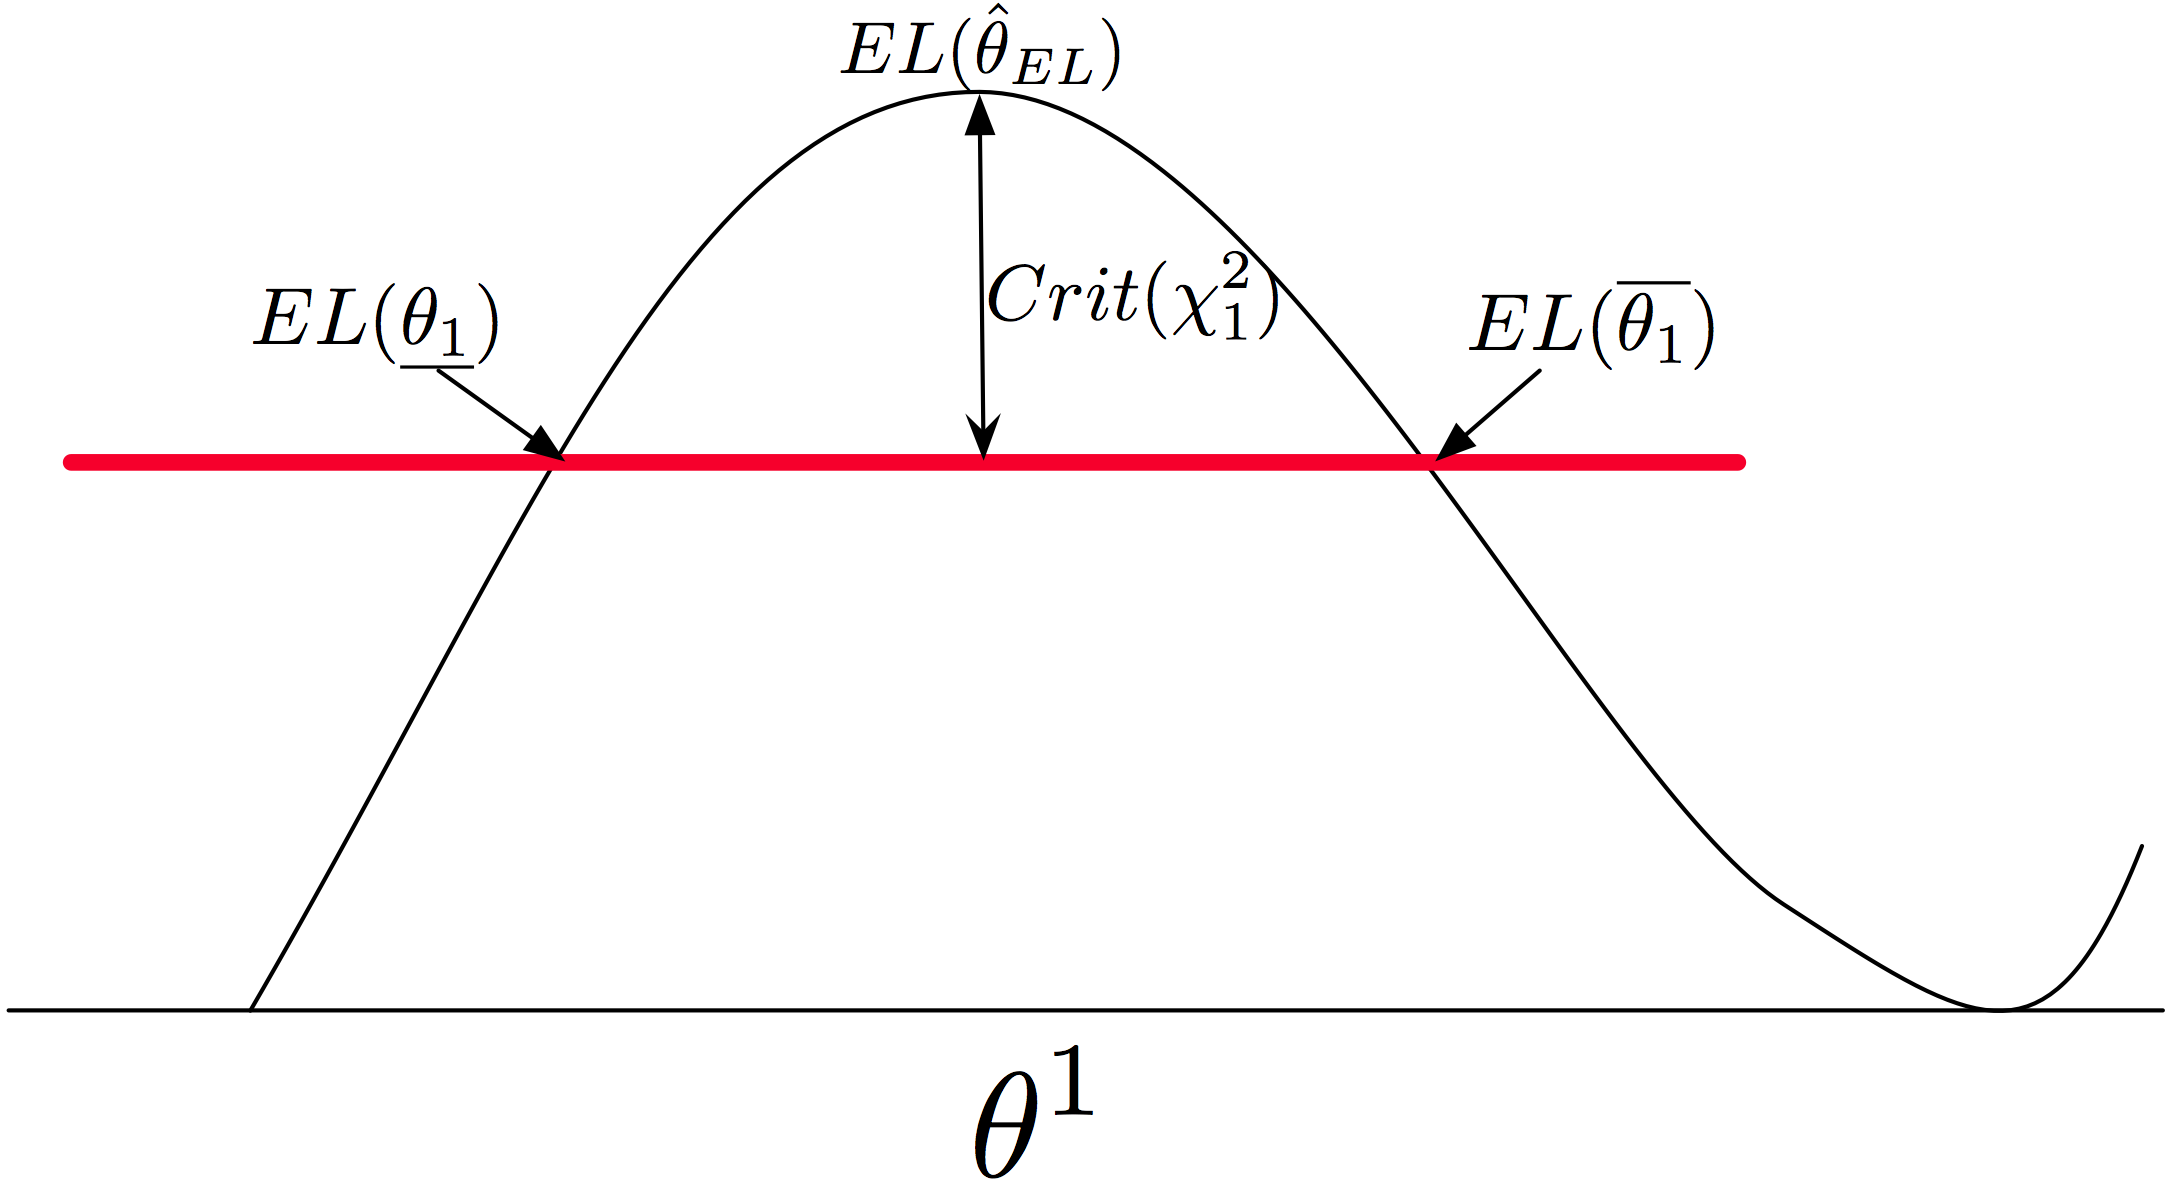
\includegraphics[width=4.5in]{resources/elci.png}
\label{default}
\end{center}
\end{figure}
}


\subsection{Example}
\frame{\frametitle{Altonji Segal 1996 / Abowd Card 1989}
The dataset (PSID) tracks 1536 individuals over ten years, and 210 moment conditions are constructed out of all of the possible permutations of variances, covariances, and autocovariances for different lags. A stationary model is estimated with 45 parameters. 
\begin{center}
\rowcolors[]{1}{RoyalBlue!10}{RoyalBlue!20} 
\begin{tabular}{lrrr}
&\bf{MPEC-EL}\footnote{KNITRO-AMPL} & \bf{Dual}\footnote{KNITRO-AMPL  w/ Numerical Outer Loop Gradient} & \bf{ELike-M}\footnote{fminsearch-MATLAB} \\
Moments &210 &210 &210\\
Parameters & 1591& 255 (45)& 255(45) \\
Iterations & 65 & 1023 & 10,000+ \\
\# Converged & 50 & 46 & 42 \\
Time & $\approx 25 s$ & $\approx$ 20 m  & $\approx$ 45 m\\
\end{tabular}
\end{center}}


\subsection{BLP MPEC}
\frame{\frametitle{Dube Fox Su 2009}
An MPEC Algorithm for computing the same estimator as BLP has been suggested:
\begin{exampleblock}{BLP-MPEC}
The estimator solves the following mathematical program:
\begin{eqnarray*}
\label{blpmpec}
\min_{\theta, \xi,s,g}  && g(\xi)' W g(\xi) \quad \mbox{ s.t. } \\
g(\xi) &=& \frac{1}{N} \sum_{\forall j,t} \xi_{jt} ' z_{jt} \\
s_{jt}(\theta) &=&  \int \frac{\exp[x_{jt} \beta_i + \xi_{jt} - \alpha_i p_{jt} ]}{1 + \sum_k \exp[ x_{kt} \beta_i + \xi_{kt} - \alpha_i p_{kt} ]} f(\beta_i | \theta)\\
\log(S_{jt})  &=& \log(s_{jt}(\beta,\alpha,\xi,\theta)) \quad \forall j,t
\end{eqnarray*}
\end{exampleblock}
}





\section{Nevo Example}
\subsection{(Knittel Metaxoglou 2008)}
\frame{\frametitle{(Knittel Metaxoglou 2008)}
Recent paper (just updated) takes 10 algorithms, 50 starting values and uncovers 100+ parameter estimates and Nevo code/data:
\begin{itemize}
\item \textit{a local minimum may yield parameter values that are close to the true values but have an objective function value that is very different.  Therefore we focus on the economic meaning of the variation in parameter estimates...}
\item \textit{... researchers will need to use multiple starting values, at least 50 and multiple algorithms}
\item Mistakes abound
\item What weight matrix is used?
\end{itemize}
}

\frame{\frametitle{Nevo Results}
\begin{center}
\rowcolors[]{1}{RoyalBlue!5}{RoyalBlue!15} 
\begin{tabular}{lrrrr}
& Nevo & BLP-MPEC & EL\\
Price& -28.189  & -62.726  & -61.433  \\
$\sigma_{p}$ &0.330 & 0.558 & 0.524\\
$\sigma_{const}$ &2.453 &3.313 & 3.143\\
$\sigma_{sugar} $& 0.016&-0.006 & 0\\
$\sigma_{mushy} $&0.244 &0.093&0.085\\
$\pi_{p,inc}$ &15.894  &588.206 & 564.262\\
$\pi_{p,inc2}$ &-1.200  &-30.185 &-28.930 \\
$\pi_{p,kid}$ &2.634 &11.058 &   11.700\\
$\pi_{c,inc}$ &5.482 & 2.29084&2.246\\
$\pi_{c,age} $& 0.2037&1.284 & 1.37873 \\
GMM &29.3611 &4.564 & \\
EL & & &-17422  \\
Time & 28 s & 12s & 19s  \\
\end{tabular}
\end{center}
}

\frame{\frametitle{Profile Empirical Likelihood}
\begin{figure}
\begin{center}
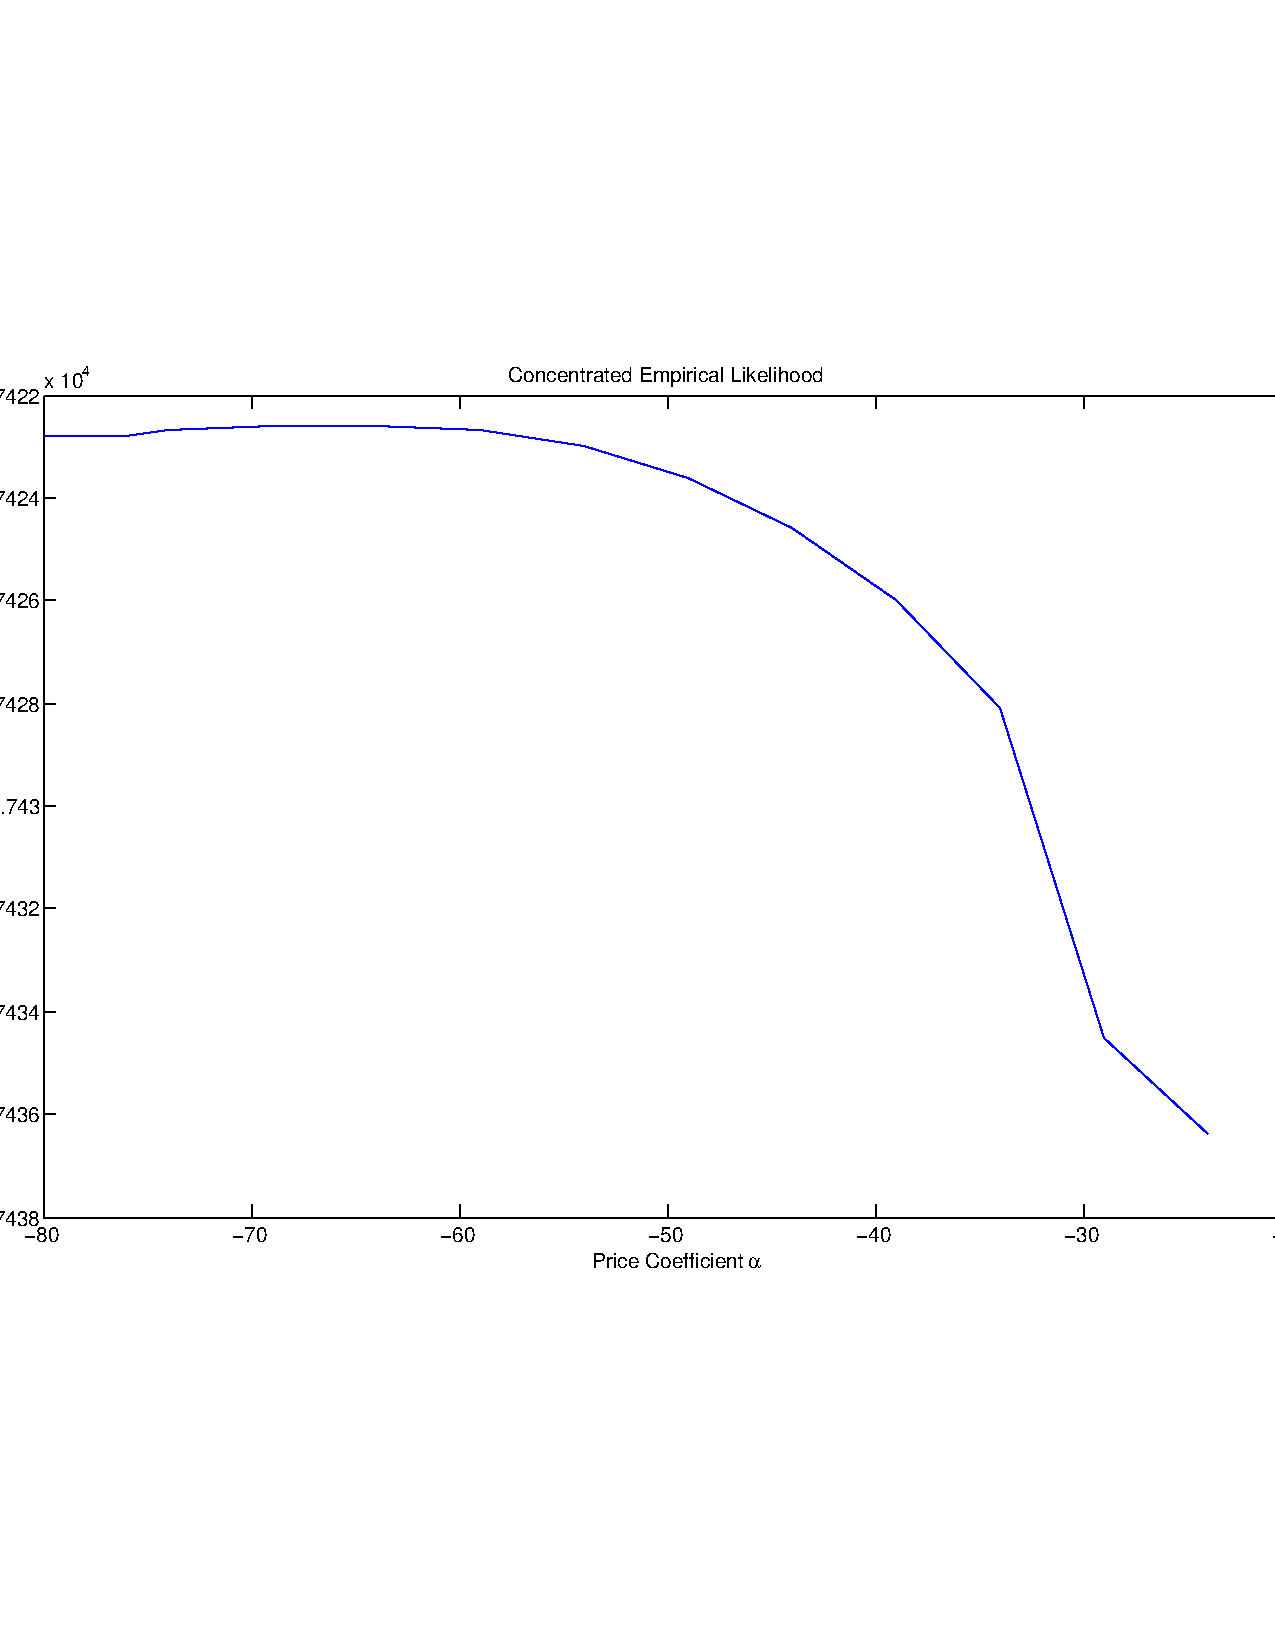
\includegraphics[width=2.5in]{resources/profileel.pdf}
\caption{Profile EL Shows Non-Identification}
\end{center}
\end{figure}
}

%\frame{\frametitle{Conditional Empirical Likelihood}
%\begin{itemize}
%\item Looks a lot like weak instruments
%\item CEL does slightly better
%\item Theory tells us that $E[\xi_{jt} | Z_{jt} ] =0$ but we usually estimate $E[\xi_{jt} Z_{jt} ] =0$ which is the weaker exogeneity restriction.
%\item The CEL curve looks a bit less flat and better identified.
%\item If you thought $n$ extra parameters was bad -- imagine $n^2$.
%\end{itemize}
%}



\end{document}


